\subsection{Runs and losses}
Tables~\ref{tab:p3t} and~\ref{tab:p3r} list every P3 run (FP32 validation loss recomputed on the saved checkpoint over the full 1000 sequence validation set; these agree with the logged bf16 values to three decimals). Transformer variants were run at $\lr\in\{0.003, 0.006\}$ (block 2 at its own centre, $\{0.0045, 0.009\}$), RNN variants at $\{0.001, 0.002\}$, and the range was extended once where the best rate sat on the edge (block 2 to 0.018, EMA 0.1 down to 0.00075).

\begin{table}[h]\centering\small
\caption{P3 transformers (d8). Best rate per variant in bold.}
\label{tab:p3t}
\begin{tabular}{lp{0.78\linewidth}}\toprule
variant & final validation loss per peak rate\\\midrule
d8 (supplied) & $\lr$=0.003: 2.927 (best of five) \\
d8-half & $\lr$=0.003: \textbf{2.933}; $\lr$=0.006: 2.938 \\
d8-ema01 & $\lr$=0.00075: \textbf{6.875}; $\lr$=0.003: 6.875; $\lr$=0.006: 6.875 \\
d8-ema09 & $\lr$=0.003: \textbf{2.950}; $\lr$=0.006: 2.969 \\
d8-uniform & $\lr$=0.003: \textbf{2.924}; $\lr$=0.006: 2.939 \\
d8-attention & $\lr$=0.003: \textbf{2.904}; $\lr$=0.006: 2.916 \\
d8-block2 & $\lr$=0.0045: 2.917; $\lr$=0.009: \textbf{2.900}; $\lr$=0.018: 3.600 \\
d8-block4 & $\lr$=0.003: 2.916; $\lr$=0.006: \textbf{2.910} \\
d8-route & $\lr$=0.003: \textbf{2.915}; $\lr$=0.006: 2.927 \\
\bottomrule\end{tabular}

\end{table}
\begin{table}[h]\centering\small
\caption{P3 modern RNNs.}
\label{tab:p3r}
\begin{tabular}{lp{0.78\linewidth}}\toprule
variant & final validation loss per peak rate\\\midrule
rnn (supplied) & $\lr$=0.002: 3.516 (best of five) \\
rnn-half & $\lr$=0.001: \textbf{3.503}; $\lr$=0.002: 3.538 \\
rnn-ema01 & $\lr$=0.001: \textbf{3.572}; $\lr$=0.002: 3.589 \\
rnn-ema09 & $\lr$=0.001: \textbf{3.505}; $\lr$=0.002: 3.512 \\
rnn-uniform & $\lr$=0.001: \textbf{3.572}; $\lr$=0.002: 3.583 \\
rnn-attention & $\lr$=0.001: 3.550; $\lr$=0.002: \textbf{3.547} \\
rnn-block2 & $\lr$=0.001: \textbf{3.535}; $\lr$=0.002: 3.577 \\
rnn-block4 & $\lr$=0.001: \textbf{3.515}; $\lr$=0.002: 3.578 \\
rnn-route & $\lr$=0.001: \textbf{3.518}; $\lr$=0.002: 3.522 \\
\bottomrule\end{tabular}

\end{table}

\paragraph{Transformer.} Replacing the additive skip is mostly a loss. EMA with $\beta=0.1$ collapses to the unigram loss 6.875 at all three rates: with $x' = 0.1x + F(N(x))$ the stream is dominated by the latest branch, the probe in Figure~\ref{fig:p3t} shows its gradient falling from $10^{-9}$ at the top to $10^{-17}$ at the bottom exactly like the no-residual model in P1, and its final stream RMS is 400. EMA $\beta=0.9$ trains but costs 0.02 to 0.04 nats (2.950) and prefers the lower rate; averaging the two previous states (half) costs 0.006 (2.933); uniform routing is neutral (2.924). Learned routing is the only change that helps: full attention residuals 2.904 at 0.003 (2.916 at 0.006), blocked attention with $B=4$ 2.910 and with $B=2$ 2.900 at $\lr=0.009$, the best transformer in this report, with 3.600 at 0.018 marking the top of its range. The routed models are the only P3 transformers that beat P1's best gate (gated residual, 2.910). My gated route variant reaches 2.915 at the baseline's rate with no retuning, 0.012 better than the baseline, but it stays behind the full and blocked attention residuals: starting from the additive solution makes it safe, and also makes it stay close to that solution.

\paragraph{RNN.} The modern RNN is less sensitive to the depth scheme because it only has eight branches. EMA 0.1 (3.572) and uniform routing (3.572) are the worst, 0.056 behind the 3.516 baseline; half (3.504) and EMA 0.9 (3.505) are slightly better than the baseline; full attention residuals (3.547) and block 2 (3.535) are worse, block 4 (3.515) matches, and the gated route is neutral (3.518). Every RNN variant prefers $\lr=0.001$, half the baseline's best rate, except full attention. The RNN routers barely specialise: the normalised entropy of their routing weights is 0.93 to 0.99 at every depth (uniform would be 1), against 0.01 to 0.33 for the first routers of the blocked transformers.

\subsection{Depth diagnostics at init, step 100 and the end}
Figures~\ref{fig:p3t} and~\ref{fig:p3r} compare the final checkpoints (Figures~\ref{fig:p3ti} and~\ref{fig:p3te} in the appendix show initialisation and step 100). The fixed mixing schemes change the stream scale: at init the half, EMA 0.9 and baseline streams grow to 1.5 to 2.3 while uniform routing holds the stream at 0.2 and the blocked variants at 0.3 to 0.6, because the router input is an average of sources rather than their sum. After training the additive, EMA 0.9 and half streams end at RMS 12 to 24, the blocked and uniform ones at 1.4 to 5.6, and their branches write 3 to 5 times their input (against 0.3 to 0.5 in the baseline): routed models keep a small stream and large updates, additive models a large stream and small updates, and both train. The gradient profiles of all routed and mixed variants are flat across depth, like the baseline's, except EMA 0.1. At the end of training my gated route model has learned a gate of about $-1$ on the first branch, so the first attention block receives an input of RMS $10^{-3}$ and acts as a nearly constant offset while the embedding reaches later blocks through the additive stream; the remaining gates stay small and the final read puts 16\% of its weight on the output of block 3 and spreads the rest. The blocked transformers put 29\% (B=2) and 37\% (B=4) of their final read on the last block sum and 10 to 19\% on the embedding, that is, they learn a skip from the embedding to the head.

\begin{figure}[h]\centering
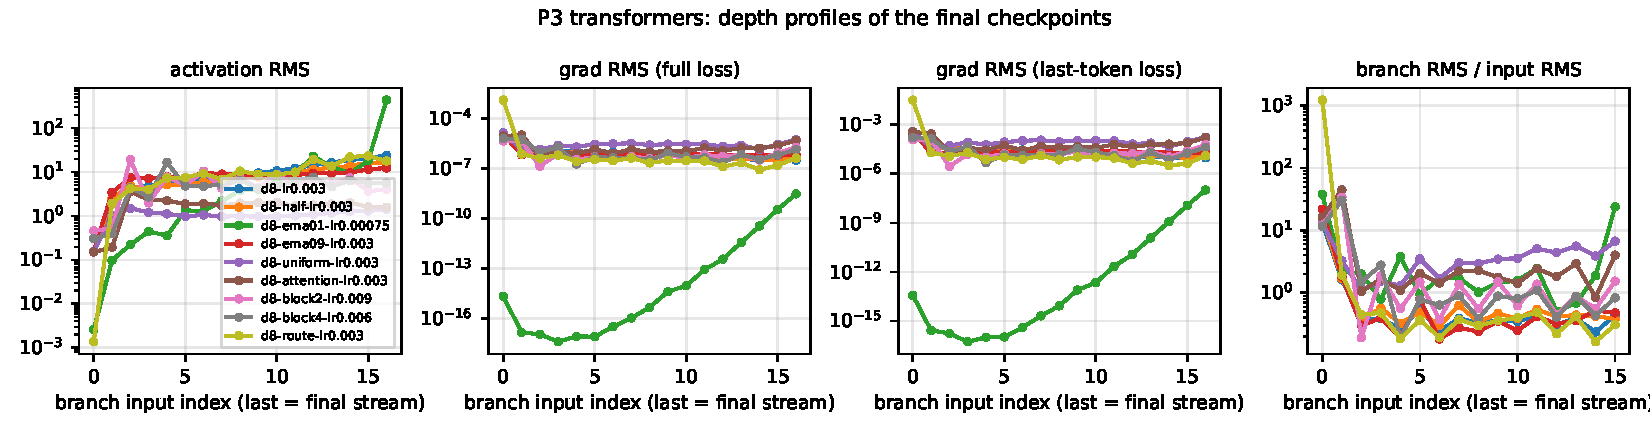
\includegraphics[width=\linewidth]{p3_t_depth_final.pdf}
\caption{P3 transformers: final checkpoints at each variant's best rate.}
\label{fig:p3t}
\end{figure}
\begin{figure}[h]\centering
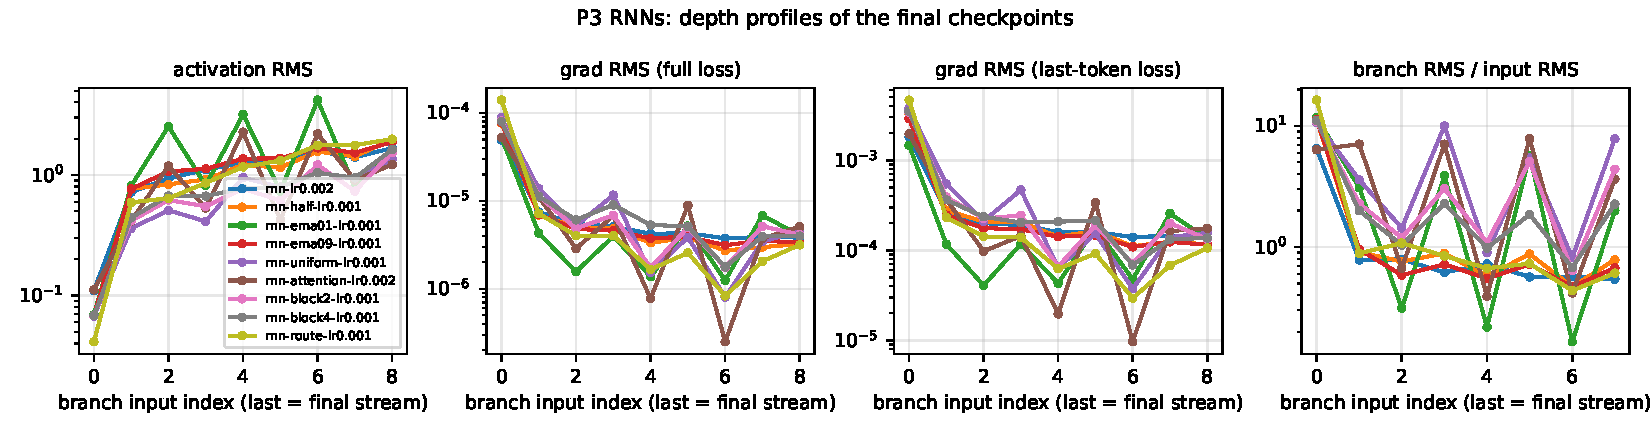
\includegraphics[width=\linewidth]{p3_r_depth_final.pdf}
\caption{P3 modern RNNs: final checkpoints at each variant's best rate.}
\label{fig:p3r}
\end{figure}
\begin{figure}[h]\centering
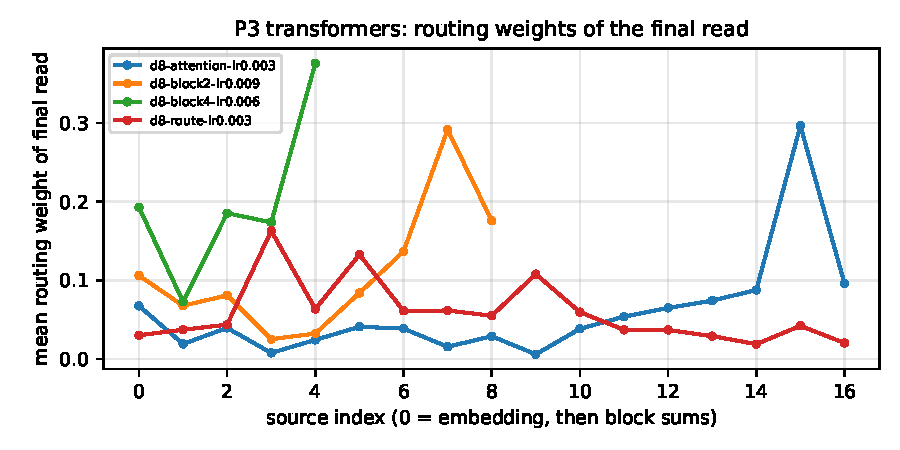
\includegraphics[width=.6\linewidth]{p3_t_routing.pdf}
\caption{Mean routing weights of the final read for the routed transformers.}
\label{fig:p3route}
\end{figure}
